%% LyX 2.3.5.2 created this file.  For more info, see http://www.lyx.org/.
%% Do not edit unless you really know what you are doing.
\documentclass[conference]{IEEEtran}
\usepackage{amsmath}
\usepackage{amssymb}
\usepackage{fontspec}
\usepackage{float}
\usepackage{graphicx}

\makeatletter

%%%%%%%%%%%%%%%%%%%%%%%%%%%%%% LyX specific LaTeX commands.
%% Because html converters don't know tabularnewline
\providecommand{\tabularnewline}{\\}
%% A simple dot to overcome graphicx limitations
\newcommand{\lyxdot}{.}


%%%%%%%%%%%%%%%%%%%%%%%%%%%%%% User specified LaTeX commands.
\IEEEoverridecommandlockouts
% The preceding line is only needed to identify funding in the first footnote. If that is unneeded, please comment it out.
\usepackage{cite}
\usepackage{amsfonts}\usepackage{algorithmic}
\usepackage{textcomp}
\usepackage{xcolor}
\def\BibTeX{{\rm B\kern-.05em{\sc i\kern-.025em b}\kern-.08em
    T\kern-.1667em\lower.7ex\hbox{E}\kern-.125emX}}

\makeatother

\begin{document}
\title{ELL409 Assignment 1}
\author{\IEEEauthorblockN{Harman Singh} \and \IEEEauthorblockN{Aayush Srivastava} }
\maketitle
\begin{abstract}
Solutions for Assignment 3 of ELL409. 
\end{abstract}


\section{Q1 SVM on health data}

We first ran PCA on the health data which has 3 features and ran SVM
to classify into the 2 classes.Then to make the decision boundaries,
we changed the problem as suggested on piazza and took the first 2
principal components of the data to. We fit SVM's with multiple kernels
and plot the decision boundaries. We also implement the SMO algorithm
and compare its performance, training time with libSVM.

\subsection{Running SVM with different Kernels}

\subsection{Decision Boundaries}

Decision boundaries for all kernels (Linear, RBF, polynomia with different
degrees) is shown in Figure \ref{fig:Question1_fig1}. These figures
correspond to the optimal values of 'C' and gamma (in case of RBF)
kernel. The yellow dots signify that they are support vectors. 

\begin{figure}[H]
\begin{centering}
\includegraphics[width=0.9\columnwidth]{images/Q1\lyxdot 3supportvecs_decision}
\par\end{centering}
\caption{Decision boundary for various kernels \label{fig:Question1_fig1}}
\end{figure}


\subsection{Decision Boundaries with removed support vectors}

We removed the old support vectors and then ran the SVM again to fit
it to the remaining dataset. Our decision boundaries are as shown
in Figure \ref{fig:Question1_fig2}. The yellow marked points are
the new support vectors. As we can see these are much smaller in number.

\begin{figure}[H]
\begin{centering}
\includegraphics[width=0.9\columnwidth]{images/Q1\lyxdot 3without_supportvecs_decision}
\par\end{centering}
\caption{Decision boundary for various kernels when old support vectors are
removed \label{fig:Question1_fig2}}
\end{figure}


\subsection{Implementing SMO algorithm (bonus part)}

We referred to Platt's original paper, P.S.Sastri's tutorial and CS231
notes and implemented the SMO algorithm in python itself. The performance
of our code was comparable to the sklearn's LIBSVM implementation
in terms of accuracy but time taken by our code was larger.
\begin{itemize}
\item The time taken by our code was more than that of the LIBSVM as shown
in Figure \ref{fig:Question1_fig3} a) and it continues to increase
as the data scales.
\item The accuracy of LIBSVM and our implementation of SMO isplotted and
we can see that for a large enough dataset they are nearly equal to
each other (Figure \ref{fig:Question1_fig3} b))
\end{itemize}
We feel that ours is not the most optimal implementation of the algorithm
and many more techniques can be used for eg in choosing the 2 vectors
at each step and in other parts of the code. We also feel that LIBSVM
may have been implemented in C/C++ which makes it much faster than
some parts of our code in Python (like loops etc) which cannot be
vectorized using numpy arrays and hence have to suffer the slow-ness
of python.

\begin{figure}[H]
\begin{centering}
\includegraphics[width=0.45\columnwidth]{images/Q1\lyxdot 4timecomparison}\includegraphics[width=0.45\columnwidth]{images/Q1\lyxdot 4accuracycomparison}
\par\end{centering}
\caption{a)Time taken SMO implementation (smotime) vs Sklearn's LIBSVM (svmtime)
and b) accuracy of SMO implemenation (smoacc) and Sklearn's LIBSVM
(svmacc) \label{fig:Question1_fig3}}
\end{figure}


\section{Neural Networks}

\subsection{Ordinary Least Squares}

\section{Learning++}

Part A to E correspond to the 5 subquestions of Q3 

\subsection{Class Imbalance in MNIST}

MNIST class 0, 1, 2 were considered in the ratio 70:25:5. We first
used a comparitively larger self made (non standard) neural network
which gave close to 100\%(>99.8 on both train and test datasets) accuracy.
This neural network was large for the MNIST dataset and was able to
generalize well despite the class imbalance.

We then used a smaller feedforward neural network with 2 hidden layers
to first visualize the problems that arose due to class imbalance
and then try to solve them. We first tried out the following methods
and modifications to our losses.
\begin{itemize}
\item Cross entropy loss: We did not modify the loss in this case and the
results we obtained are shown in the folloing table having precision
recall and F1 score for all three classes. (Table \ref{tab3.1})
\end{itemize}
\begin{table}[H]
\begin{centering}
\begin{tabular}{c|c|c|c}
\textbf{Class} & \textbf{Precision} & \textbf{Recall} & \textbf{F1}\tabularnewline
\hline 
0 & 0.955 & 0.998 & 0.976\tabularnewline
\hline 
1 & 0.955 & 0.995 & 0.975\tabularnewline
\hline 
2 & \textbf{0.995} & \textbf{0.908} & \textbf{0.949}\tabularnewline
\hline 
Macro F1 &  &  & \textbf{0.967}\tabularnewline
\hline 
\end{tabular}
\par\end{centering}
\centering{}\caption{Simple Cross entropy loss \label{tab3.1}}
\end{table}

Missclassified samples are as follows, these are randomly picked misclassified
samples and as we can see most of them are from the class 2 which
has the least samples (Figure \ref{fig3.1})

\begin{figure}[H]
\begin{centering}
\includegraphics[width=0.9\columnwidth]{images/Fig3\lyxdot 1Missclassifiedsamples}
\par\end{centering}
\caption{Missclassified samples, random. T=True, P =Predicted\label{fig3.1}}
\end{figure}

\begin{itemize}
\item Weighted Cross entropy loss: We gave more wight to the class with
fewer sample. The weights are inversely proportional to the ratio
of classes. We get an increase in the performance metrics, particularly
the F1 score of the class 1 and 2 which have less samples. results
are as follows.(Table \ref{tab3.2})
\end{itemize}
\begin{table}[H]
\begin{centering}
\begin{tabular}{c|c|c|c}
\textbf{Class} & \textbf{Precision} & \textbf{Recall} & \textbf{F1}\tabularnewline
\hline 
0 & 0.976 & 0.996 & 0.985\tabularnewline
\hline 
1 & 0.977 & 0.997 & 0.986\tabularnewline
\hline 
2 & \textbf{0.992} & \textbf{0.951} & \textbf{0.972}\tabularnewline
\hline 
Macro F1 &  &  & \textbf{0.981}\tabularnewline
\hline 
\end{tabular}
\par\end{centering}
\centering{}\caption{Weighted cross entropy loss stats \label{tab3.2}}
\end{table}

\begin{itemize}
\item Focal loss: We experiemnted with the focal loss and obtained an increase
in performance metrics, when compared with the vanilla cross entropy
loss.(Table \ref{tab3.3})
\end{itemize}
\begin{table}[H]
\begin{centering}
\begin{tabular}{c|c|c|c}
\textbf{Class} & \textbf{Precision} & \textbf{Recall} & \textbf{F1}\tabularnewline
\hline 
0 & 0.977 & 0.995 & 0.987\tabularnewline
\hline 
1 & 0.981 & 0.997 & 0.988\tabularnewline
\hline 
2 & \textbf{0.993} & \textbf{0.965} & \textbf{0.980}\tabularnewline
\hline 
Macro F1 &  &  & \textbf{0.985}\tabularnewline
\hline 
\end{tabular}
\par\end{centering}
\centering{}\caption{Focal loss stats \label{tab3.3}}
\end{table}

\begin{itemize}
\item MSE loss: Simple MSE loss was tried out, performance is much worse
than cross entropy loss.(Table \ref{tab3.4})
\end{itemize}
\begin{table}[H]
\begin{centering}
\begin{tabular}{c|c|c|c}
\textbf{Class} & \textbf{Precision} & \textbf{Recall} & \textbf{F1}\tabularnewline
\hline 
0 & 0.863 & 0.997 & 0.925\tabularnewline
\hline 
1 & 0.853 & 0985 & 0.914\tabularnewline
\hline 
2 & \textbf{0.996} & \textbf{0.685} & \textbf{0.811}\tabularnewline
\hline 
Macro F1 &  &  & \textbf{0.8894}\tabularnewline
\hline 
\end{tabular}
\par\end{centering}
\centering{}\caption{Simple MSE loss stats \label{tab3.4}}
\end{table}

\begin{itemize}
\item Weighted MSE: Similar to Weghted Crossentropy but with this time using
MSE.(Table \ref{tab3.5})
\end{itemize}
\begin{table}[H]
\begin{centering}
\begin{tabular}{c|c|c|c}
\textbf{Class} & \textbf{Precision} & \textbf{Recall} & \textbf{F1}\tabularnewline
\hline 
0 & 0.881 & 0.998 & 0.936\tabularnewline
\hline 
1 & 0.862 & 0.988 & 0.926\tabularnewline
\hline 
2 & \textbf{0.994} & \textbf{0.718} & \textbf{0.833}\tabularnewline
\hline 
Macro F1 &  &  & \textbf{0.896}\tabularnewline
\hline 
\end{tabular}
\par\end{centering}
\centering{}\caption{Weighted MSE loss stats \label{tab3.5}}
\end{table}

\begin{itemize}
\item Focal loss type weighted MSE: We took the ideas of focal loss and
used it in MSE to increase the performance of the classification.(Table
\ref{tab3.6})
\end{itemize}
\begin{table}[H]
\begin{centering}
\begin{tabular}{c|c|c|c}
\textbf{Class} & \textbf{Precision} & \textbf{Recall} & \textbf{F1}\tabularnewline
\hline 
0 & 0.872 & 0.998 & 0.930\tabularnewline
\hline 
1 & 0.859 & 0.986 & 0.918\tabularnewline
\hline 
2 & \textbf{9.993} & \textbf{0.703} & \textbf{0.823}\tabularnewline
\hline 
Macro F1 &  &  & \textbf{0.890}\tabularnewline
\hline 
\end{tabular}
\par\end{centering}
\centering{}\caption{Focal loss MSE stats\label{tab3.6}}
\end{table}


\subsection{KMeans on SVHN + classification}

\subsection{Class Imbalance in MNIST}

\subsection{Class Imbalance in MNIST}

\subsection{2D PCA, tSNE on SVHN dataset}
\begin{itemize}
\item The result of performing PCA on SVHN is as shown in Figure \ref{figQ3.5.1}.
\end{itemize}
\begin{figure}[H]
\begin{centering}
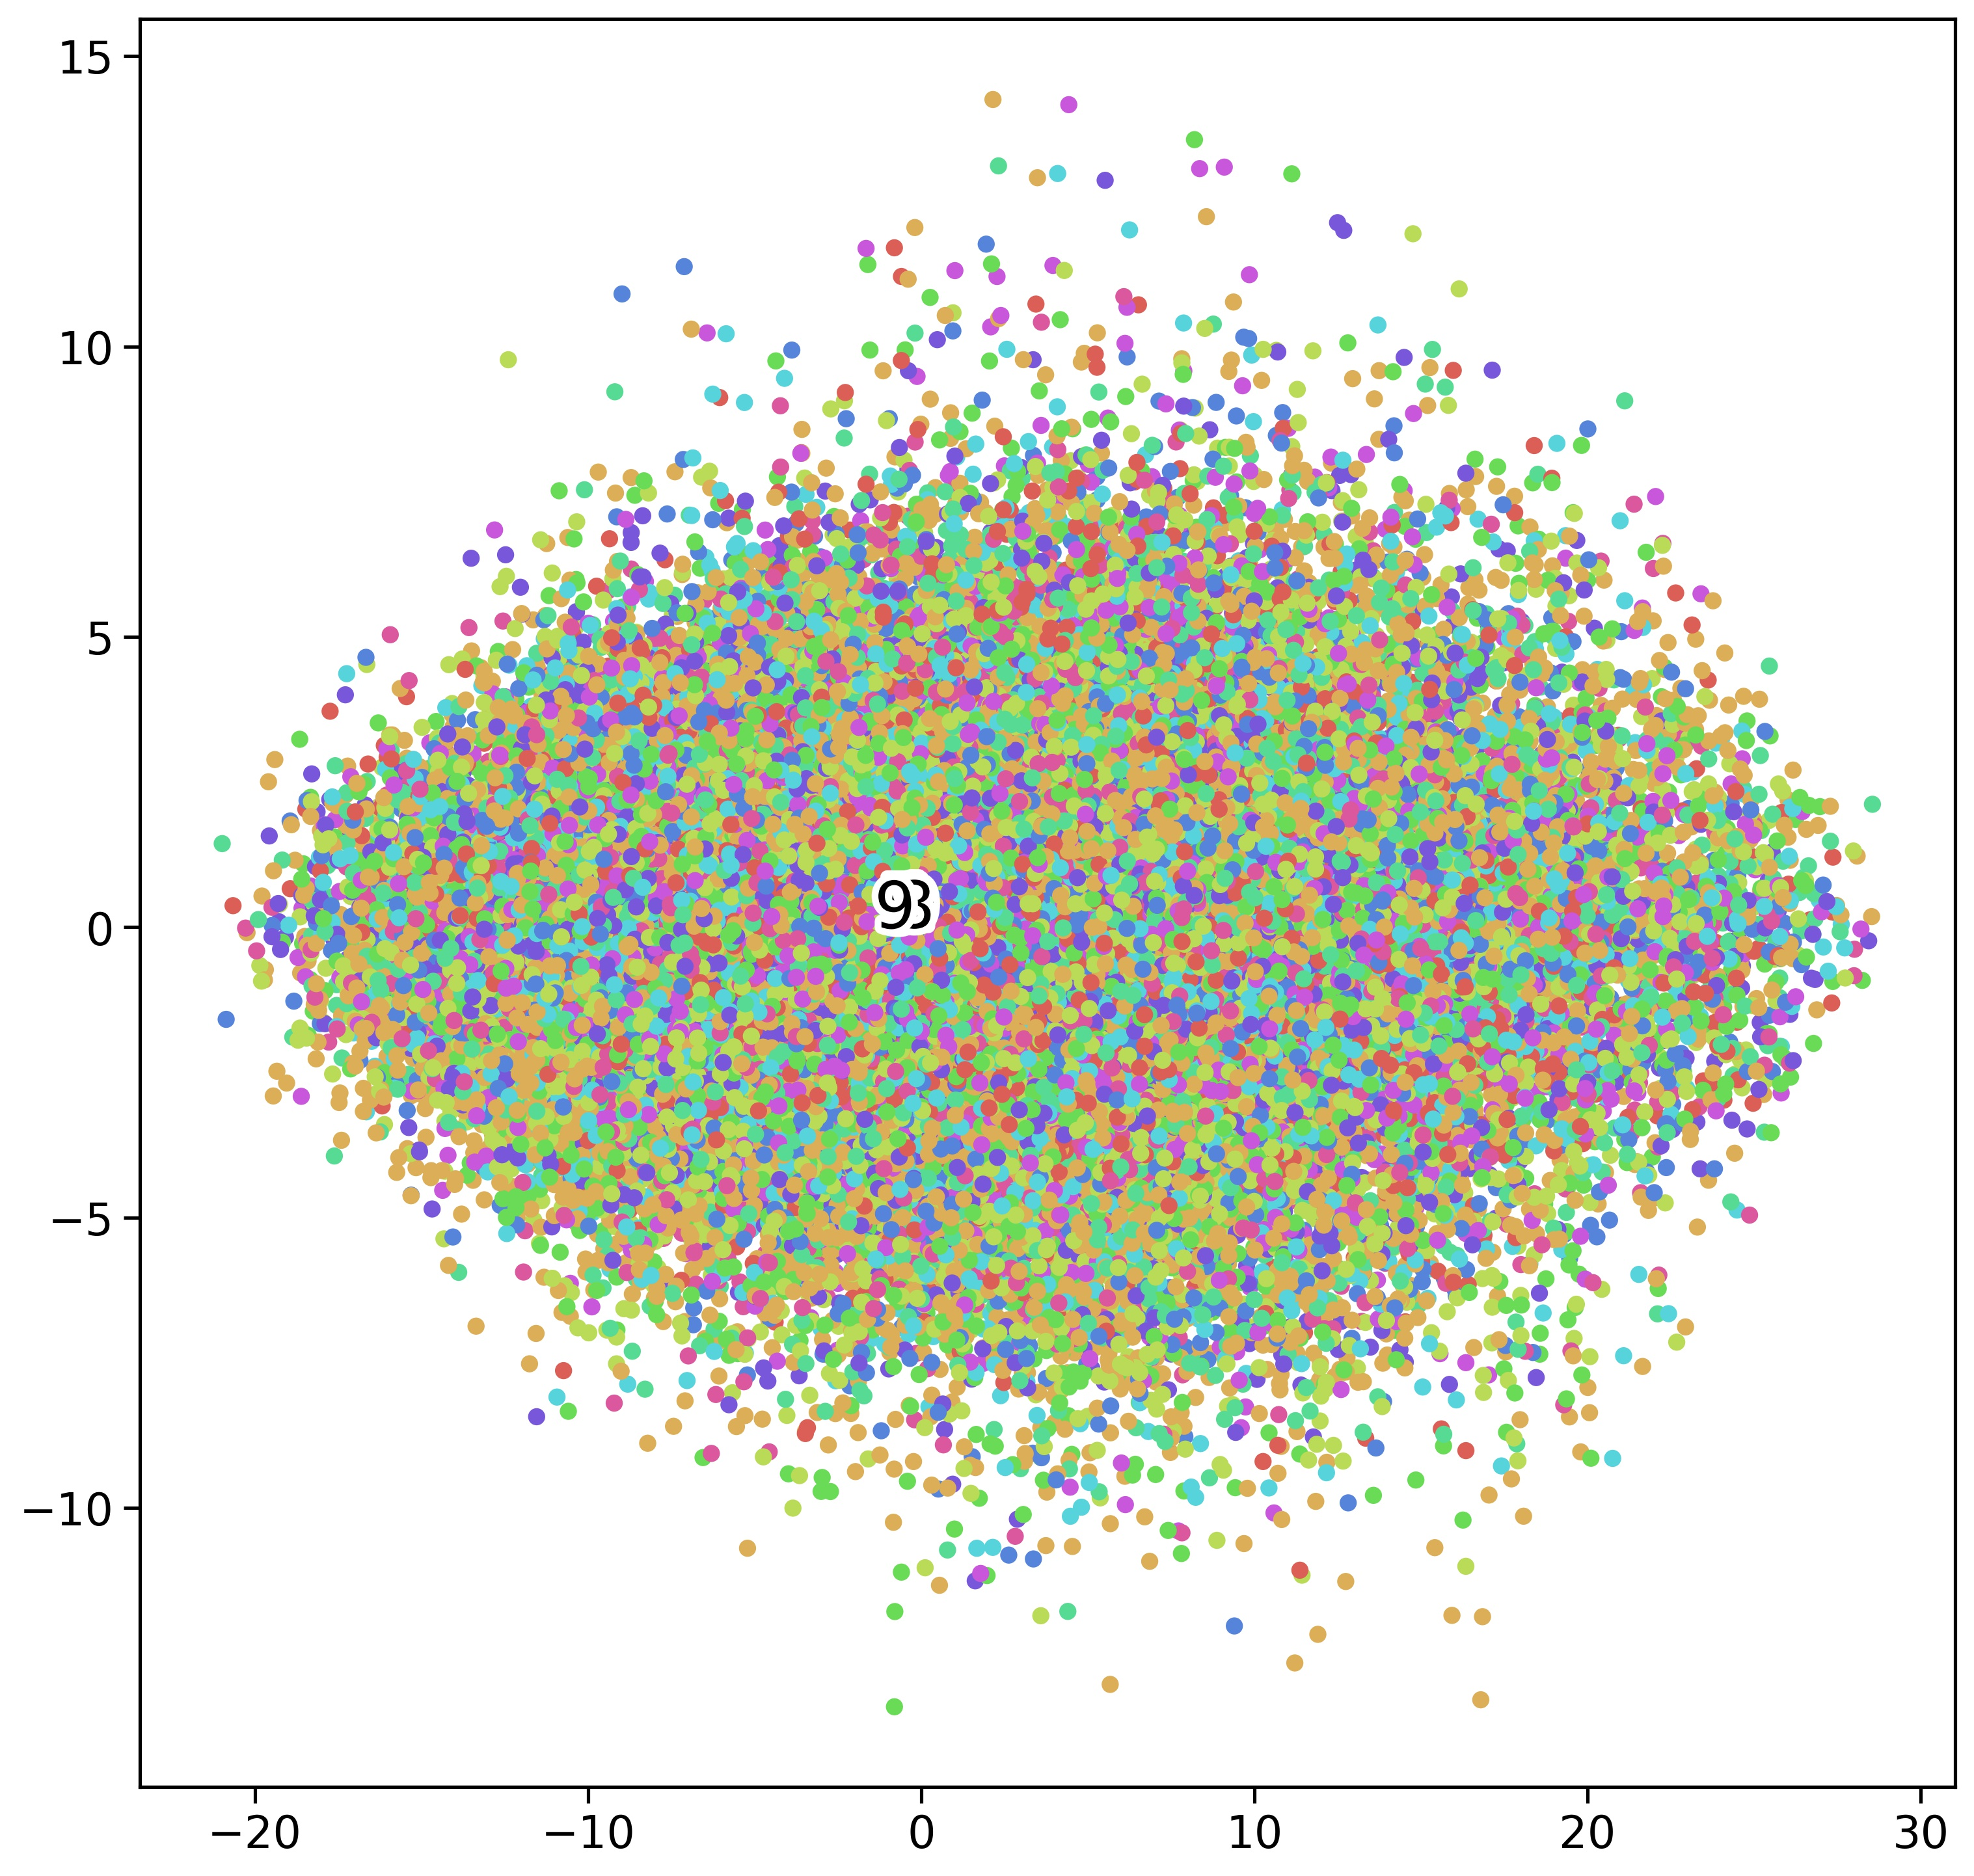
\includegraphics[width=0.9\columnwidth]{images/SVHN_PCA.jpeg}
\par\end{centering}
\caption{SVHN 2D PCA \label{figQ3.5.1}}
\end{figure}

\begin{itemize}
\item The result of performing tSNE on SVHN is as shown in Figure \ref{figQ3.5.2}.
tSNE was performed on a subset (10k images) of data which took considerable
hours on HPC.
\end{itemize}
\begin{figure}[H]
\begin{centering}
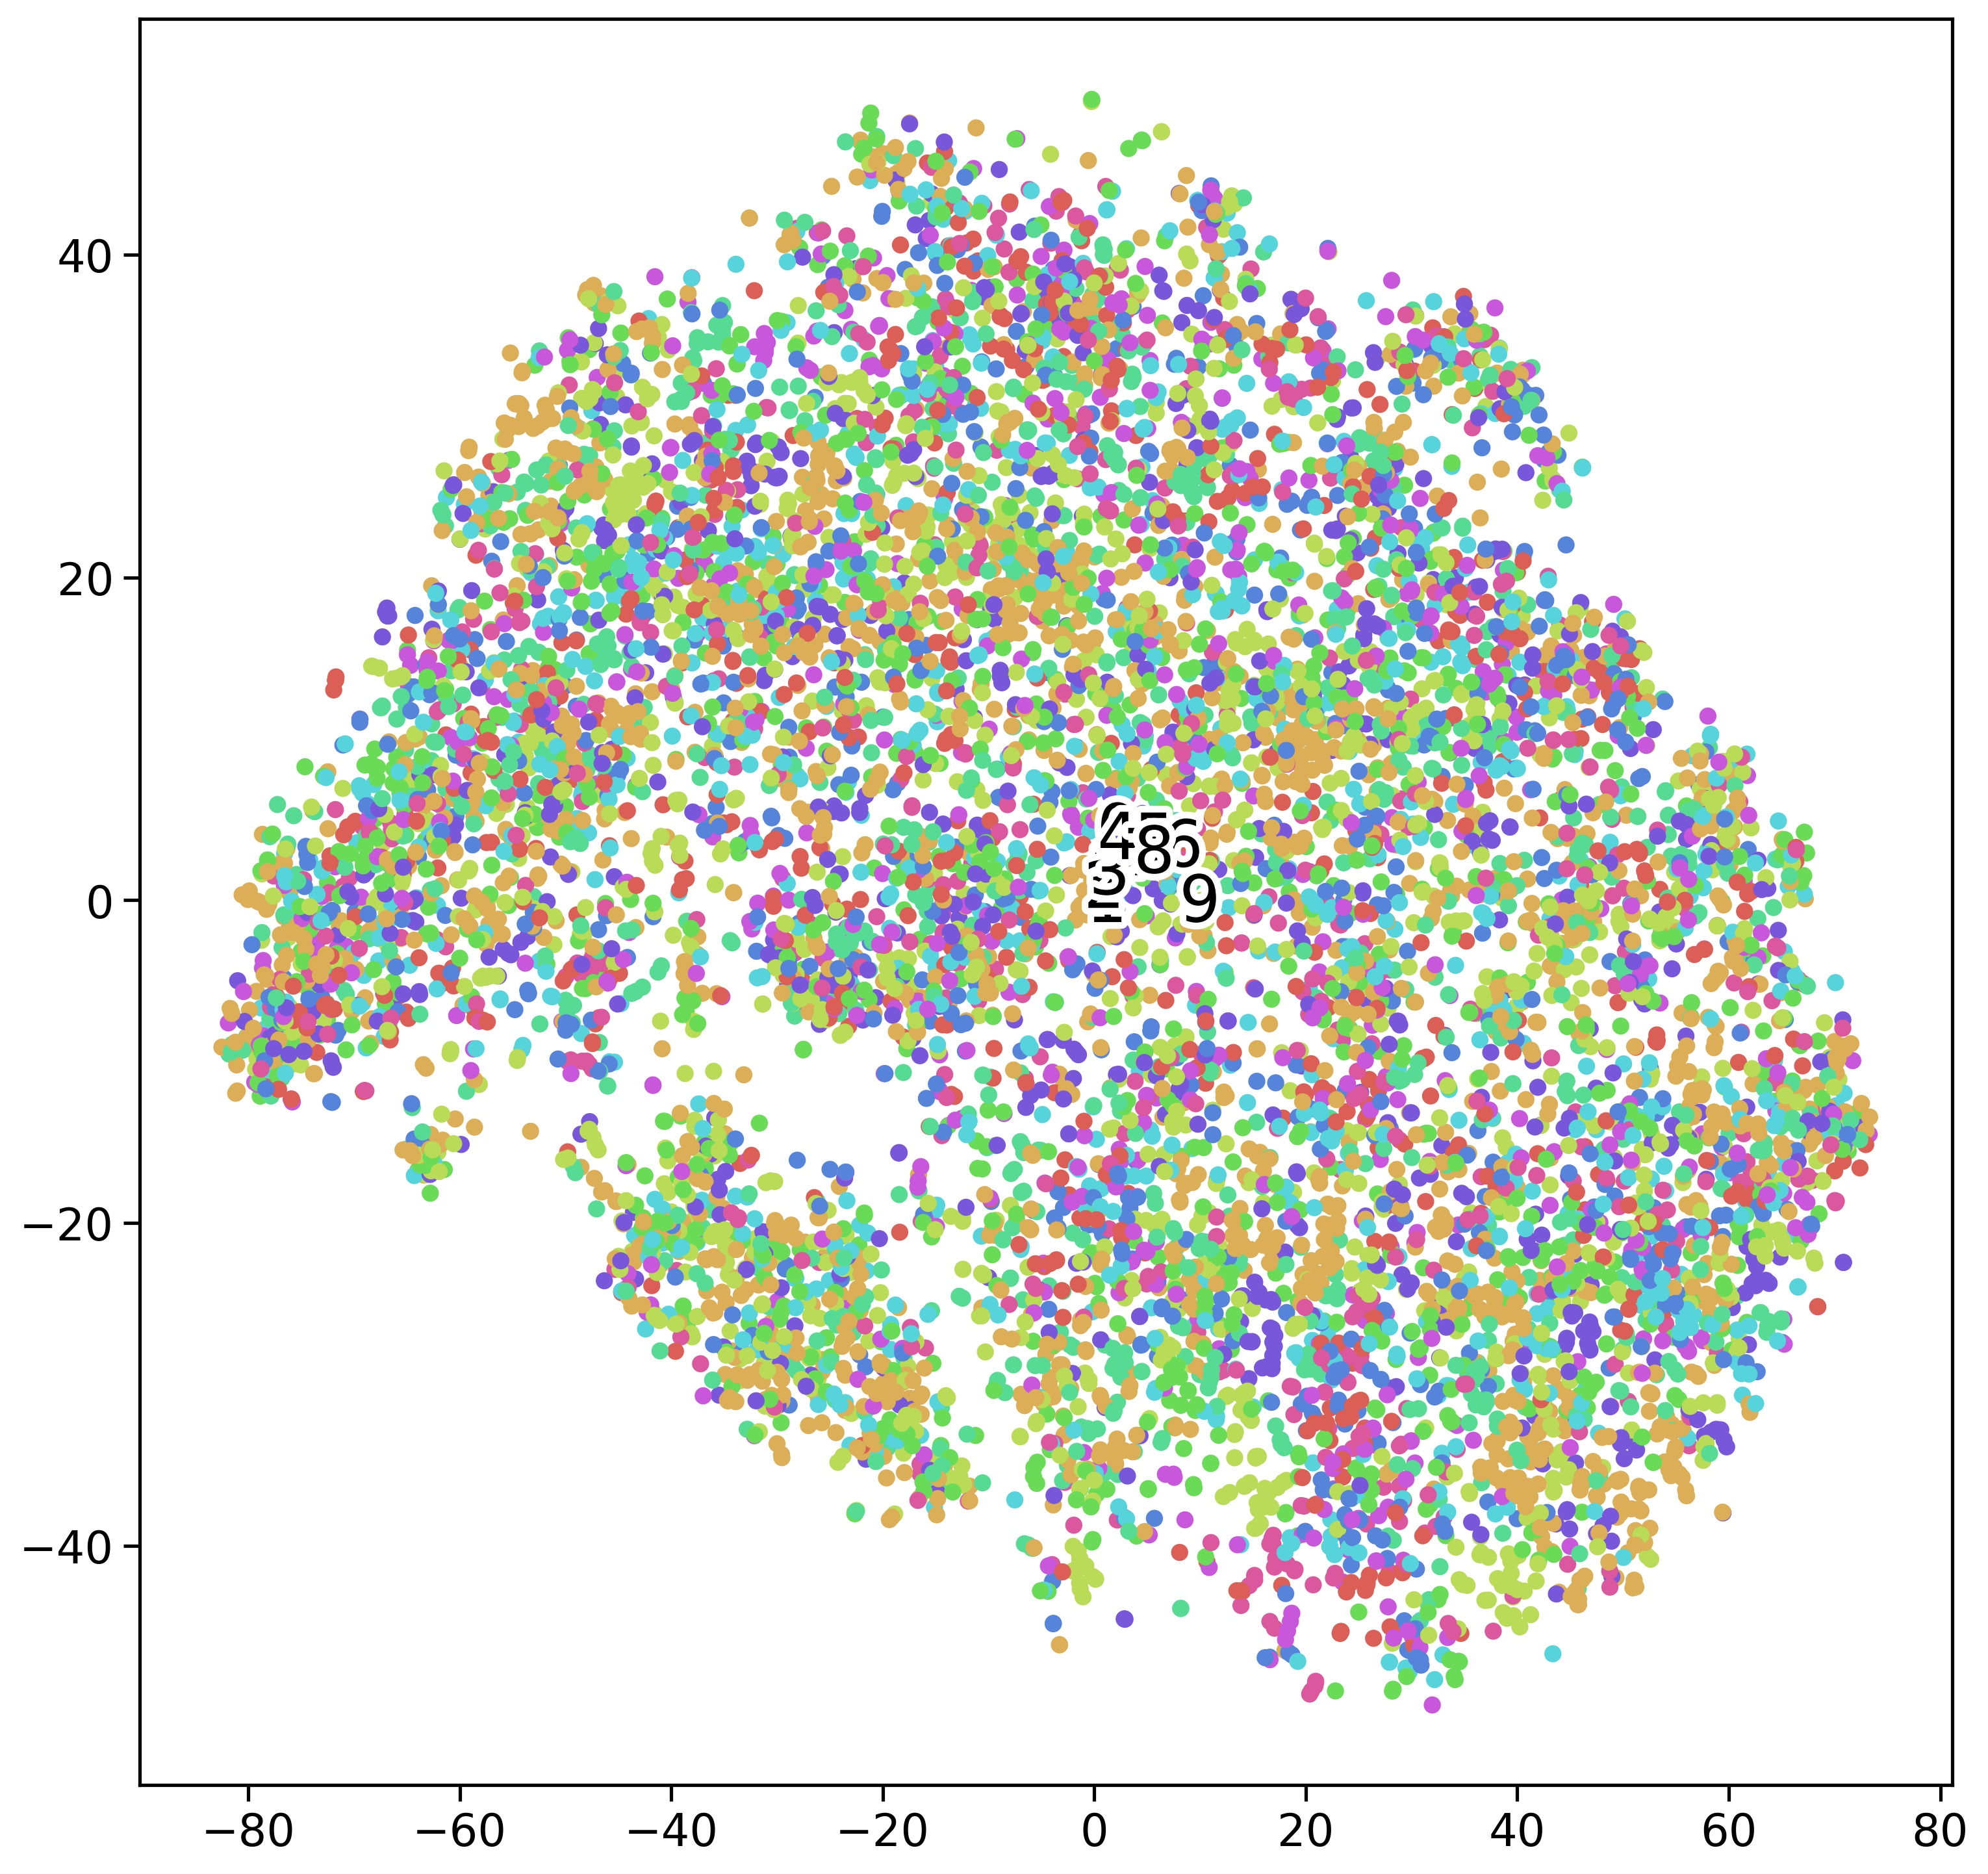
\includegraphics[width=0.9\columnwidth]{images/SVHN_tSNE.jpeg}
\par\end{centering}
\caption{SVHN 2D tSNE \label{figQ3.5.2}}
\end{figure}

\begin{itemize}
\item To have a comparison, we went ahead and performed PCA, tSNE on MNIST
data as well (Figure \ref{fig:Q3.5.3}) and based on all this we present
our observations and colnclusions below.
\end{itemize}
\begin{figure}[H]
\begin{centering}
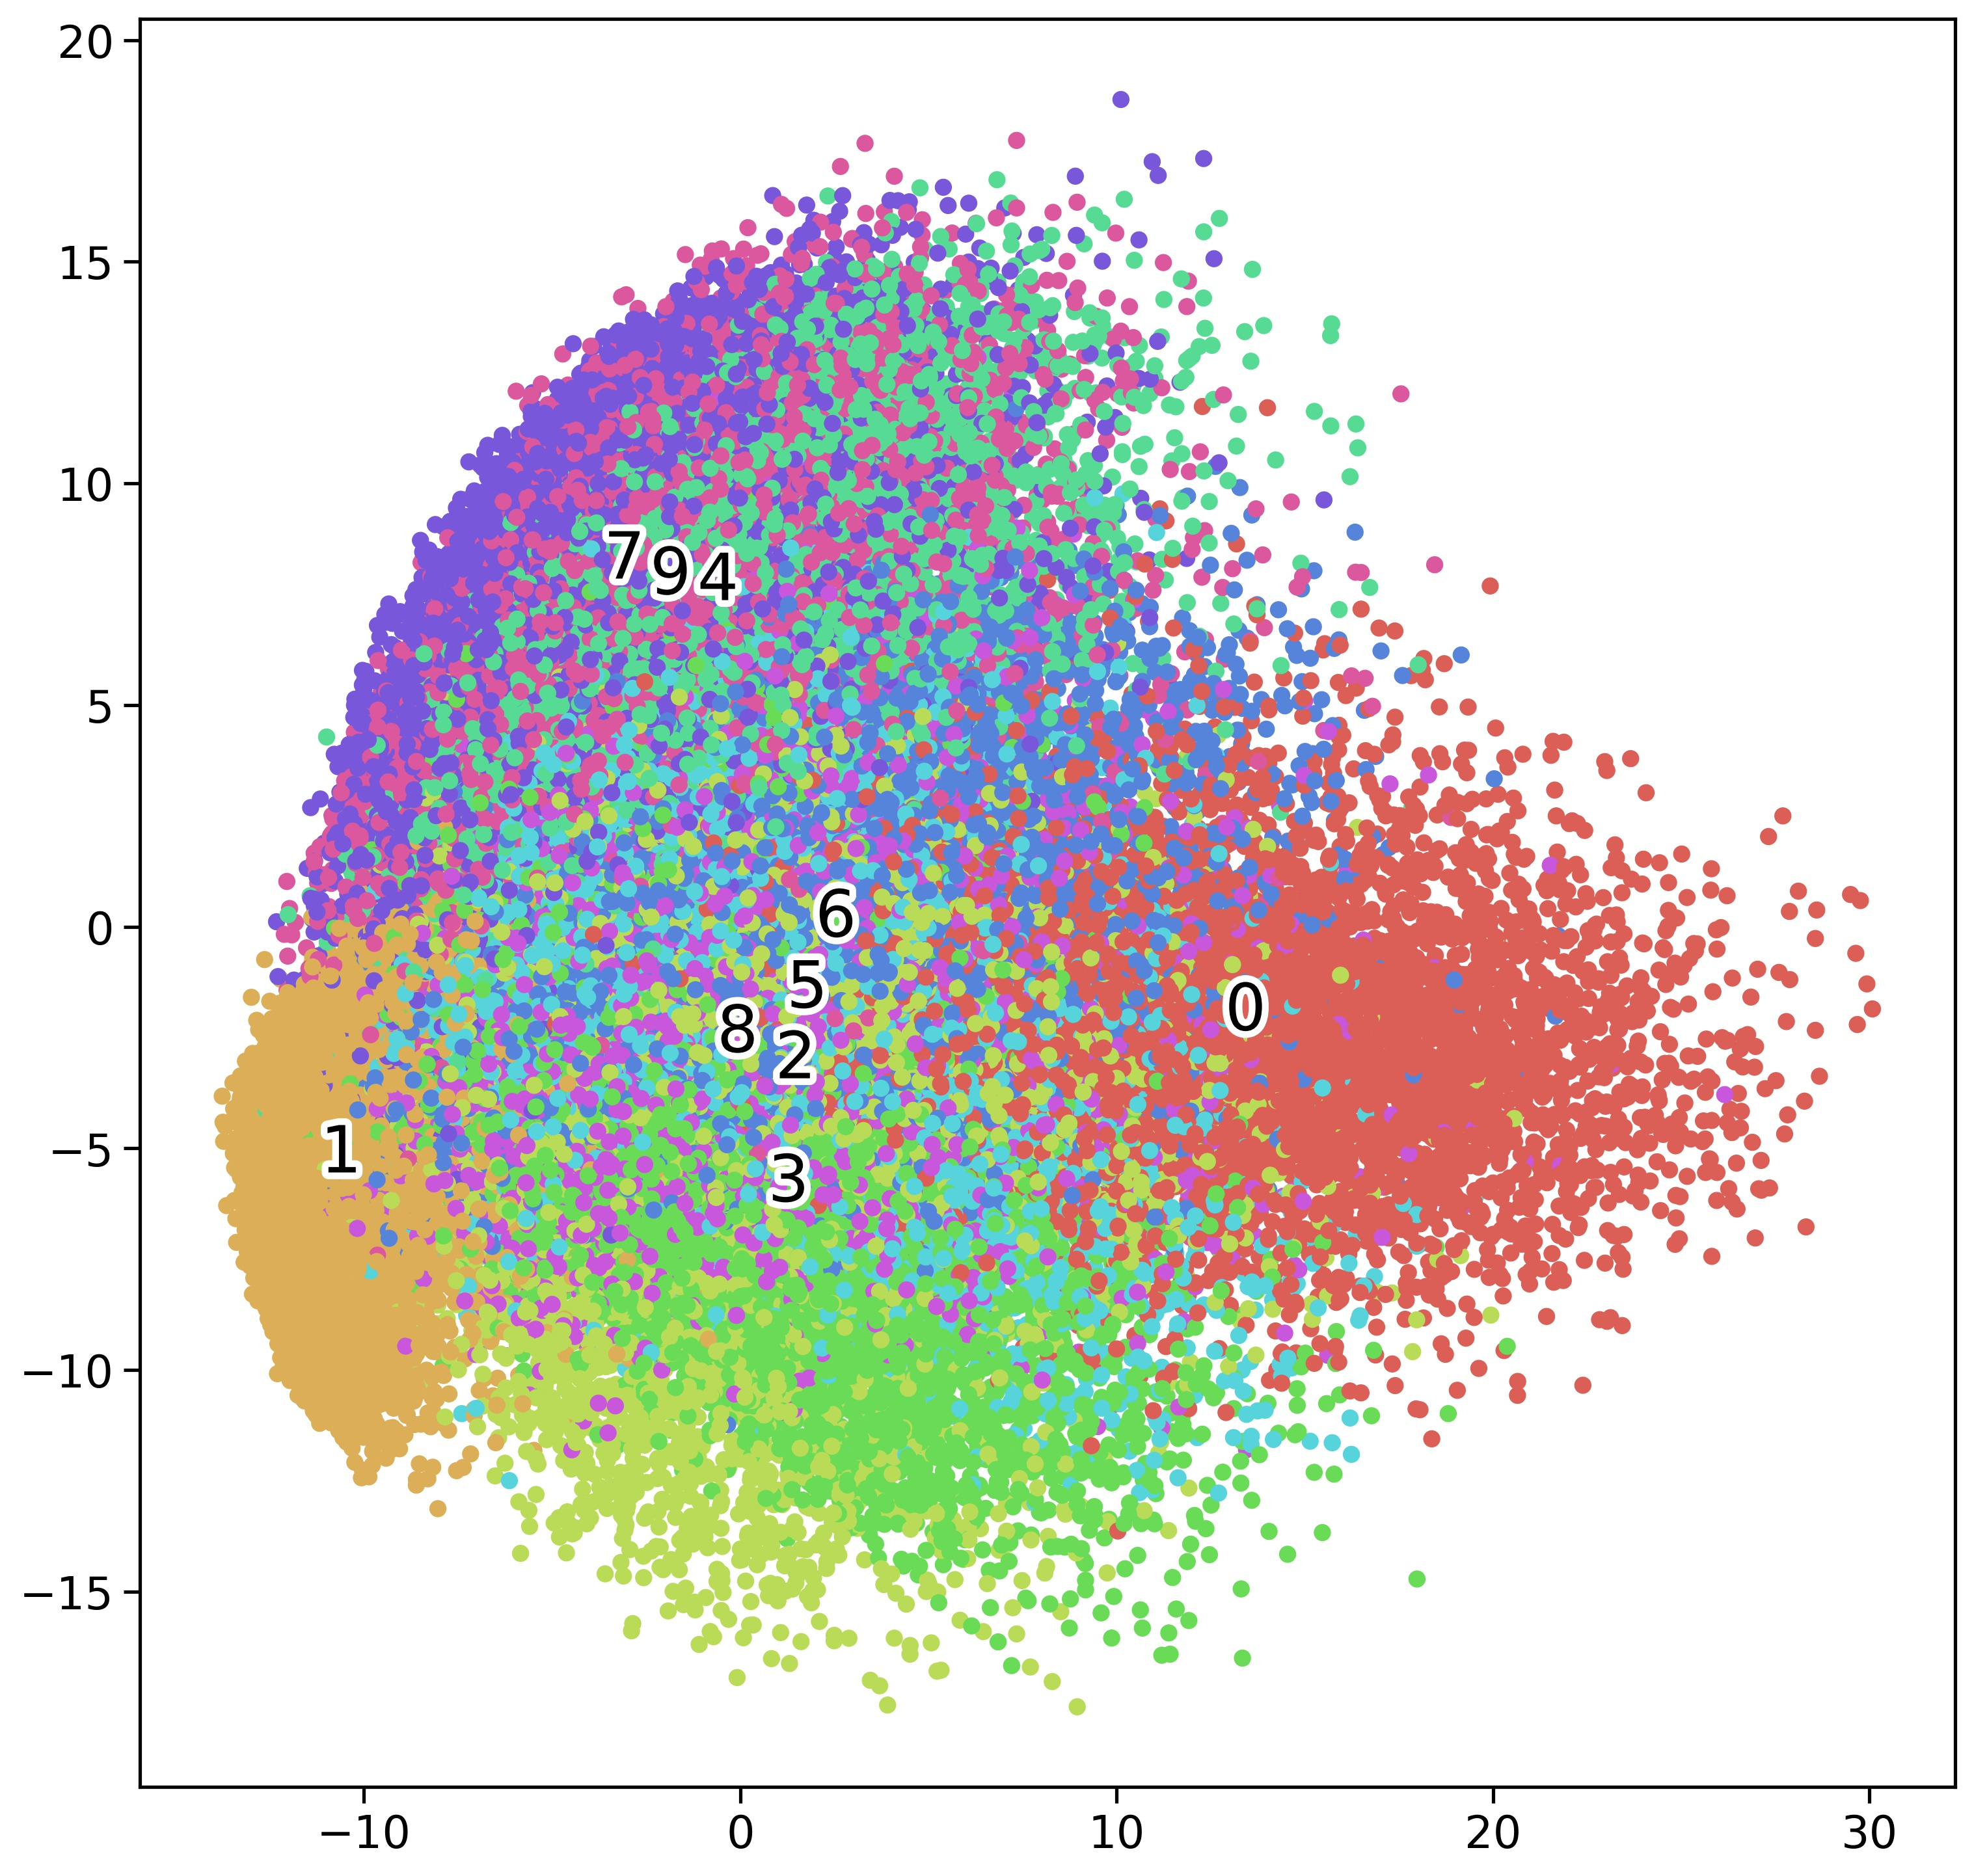
\includegraphics[width=0.45\columnwidth]{images/mnist_PCA.jpeg}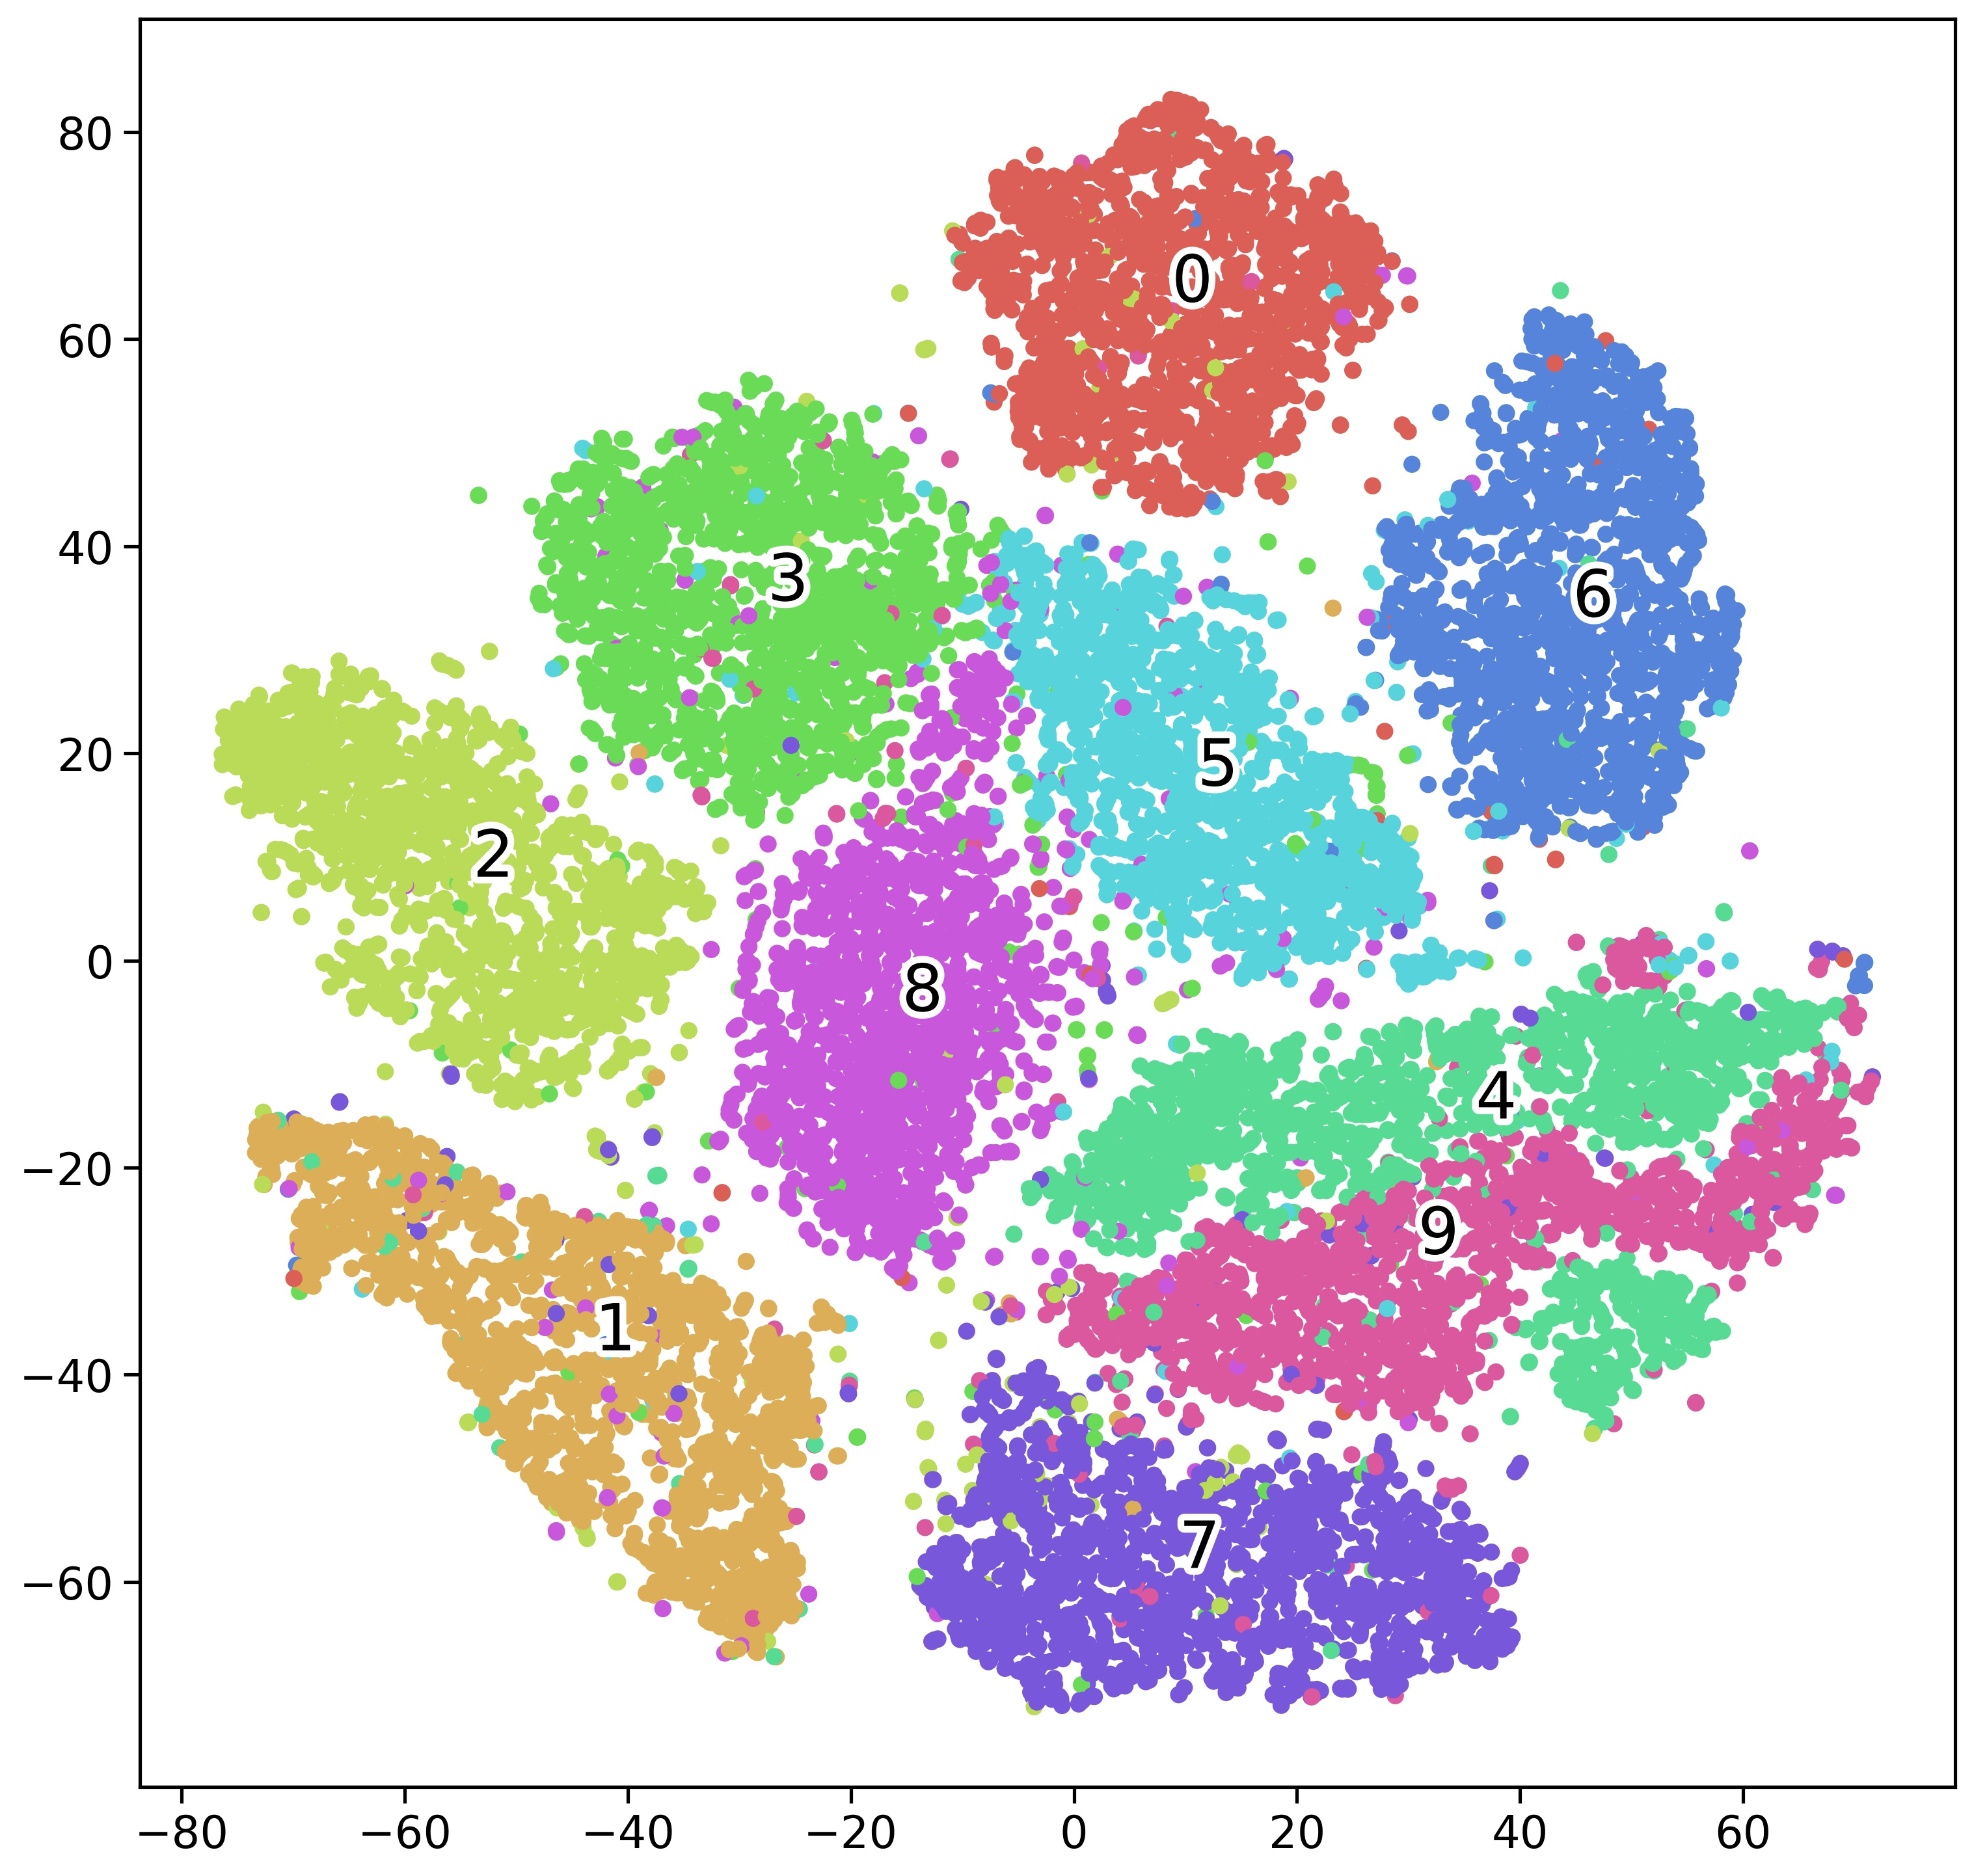
\includegraphics[width=0.45\columnwidth]{images/mnist_tSNE.jpeg}
\par\end{centering}
\caption{a)2D PCA and b)2D tSNE MNIST \label{fig:Q3.5.3}}
\end{figure}


\subsubsection{Observations and Conclusions}
\begin{itemize}
\item The PCA result on SVHN is very homogeneous, and the classes are not
separated at all. We can see that all the class labels are placed
at the same point in the figure, ie teh centroid of all the classes
is the same and hence wPCA hasn't been able to separate the classes
very well in 2 dimesnions.
\item tSNE on the other hand isn't alot better but we can ee more clustering
than PCA and the centroids of the classes are also displaced from
each other if we look closely in the tSNE plot. tSNE being a non linear
technique, it is expected that it would perform better than PCA, however
in a lot more amount of time due to (O(N\textasciicircum 2) complexity)
\item Comparing the results with MNIST we get class separationg using PCA
on MNIST. Classes 7, 9, 4 and classes 6 ,5, 8, 2 are close to each
other which is expected due to the struture of the digits. tSNE is
able to completely separate all classes from each other as shown in
the tSNE plots. An interesting thing to note is that the digit 4 is
separated into 2 groups and one is closer to 9, this is expected because
some digits, 4 look very cose to 9.
\item We can conclude that due to the noisse, background, overlapping digits
and classes, and being in more natural setting, SVHN is difficult
to separate using PCA,tSNE but MNIST is highly separable due to the
nature of the dataset, having contrast between digits and background,
uniform background, no overlapping of labels, classes etc
\end{itemize}

\subsection{smdlsk}

n param classifier, KNN, is shown here and the other one's in the
Appendix.

\begin{table}[H]
\begin{centering}
\begin{tabular}{l|l|l|l}
 & \textbf{Precision} & \textbf{Recall} & \textbf{F1}\tabularnewline
\hline 
0 & 0.996 & 0.996 & 0.996\tabularnewline
\hline 
1 & 0.995 & 0.985 & 0.99\tabularnewline
\hline 
2 & 0.994 & 0.999 & 0.996\tabularnewline
\hline 
3 & 0.97 & 0.978 & 0.974\tabularnewline
\hline 
4 & 0.967 & 0.932 & 0.949\tabularnewline
\hline 
5 & 0.953 & 0.984 & 0.969\tabularnewline
\hline 
\end{tabular}
\par\end{centering}
\begin{centering}
\begin{tabular}{l|l|l|l|l|l|l}
\hline 
 & \textbf{0} & \textbf{1} & \textbf{2} & \textbf{3} & \textbf{4} & \textbf{5}\tabularnewline
\hline 
\textbf{0} & 0.996 & 0.0 & 0.004 & 0.0 & 0.0 & 0.0\tabularnewline
\hline 
\textbf{1} & 0.0 & 0.985 & 0.0 & 0.0 & 0.001 & 0.015\tabularnewline
\hline 
\textbf{2} & 0.001 & 0.0 & 0.999 & 0.0 & 0.0 & 0.0\tabularnewline
\hline 
\textbf{3} & 0.001 & 0.0 & 0.002 & 0.978 & 0.019 & 0.0\tabularnewline
\hline 
\textbf{4} & 0.002 & 0.0 & 0.0 & 0.03 & 0.932 & 0.035\tabularnewline
\hline 
\textbf{5} & 0.0 & 0.004 & 0.0 & 0.0 & 0.012 & 0.984\tabularnewline
\hline 
\end{tabular}
\par\end{centering}
\caption{KNN on Multi-Class Dataset}
\end{table}


\appendix

\section{A}

\subsection{Binary Classification - Question 1 : Health Dataset Visualization}

\begin{figure}[H]
\begin{centering}
\includegraphics[width=7cm,height=7cm,keepaspectratio,bb = 0 0 200 100, draft, type=eps]{C:/Users/shubhammittal/Desktop/assignment/Q1_Binary_Classifier/health dataset.png}\caption{Health Data\label{fig:Health-Data}}
\par\end{centering}
\end{figure}


\subsection{Binary Classification - Question 1: Logistic Regression - Stochastic
Gradient Descent}

\begin{table}[H]

\begin{centering}
\begin{tabular}{l|l|l|l}
 & \textbf{MAE} & \textbf{MSE} & \textbf{CrossEntropy}\tabularnewline
\hline 
Val Acc & 0.8286 & 0.8469 & 0.8469\tabularnewline
\hline 
Val F1 & 0.8278 & 0.8179 & 0.8165\tabularnewline
\hline 
Train Acc & 0.851 & 0.851 & 0.851\tabularnewline
\hline 
Test Acc & 0.8714 & 0.8714 & 0.8714\tabularnewline
\hline 
Precision & 0.8571 & 0.8571 & 0.8571\tabularnewline
\hline 
Recall & 0.8478 & 0.8478 & 0.8478\tabularnewline
\hline 
F1 & 0.8525 & 0.8525 & 0.8525\tabularnewline
\end{tabular}
\par\end{centering}
\caption{Logistic Regression Classifiers with different loss functions (SGD)
\label{tab:Logistic-Regression-Classifiers-1}}

\end{table}


\subsection{Regression problem - Question 2: Elastic Net Regularization}

Here, it is seen that $\alpha$, coefficient of L2 penalty penalizes
the training loss more than $\beta$, coefficient of L1 penalty.

\begin{figure}[H]
\begin{centering}
\includegraphics[width=6cm,height=6cm,keepaspectratio,bb = 0 0 200 100, draft, type=eps]{C:/Users/shubhammittal/Desktop/assignment/Q2_Regression/ElasticNet.png}\caption{Elastic Net Regularization\label{fig:Elastic-Net-Regularization}}
\par\end{centering}
\end{figure}


\subsection{Regression problem - Question 2: Linear regression using MAE Loss
function}

\begin{figure}[H]
\begin{centering}
\includegraphics[width=5cm,height=5cm,keepaspectratio,bb = 0 0 200 100, draft, type=eps]{C:/Users/shubhammittal/Desktop/assignment/Q2_Regression/MAE_regressor.png}\includegraphics[width=5cm,height=5cm,keepaspectratio,bb = 0 0 200 100, draft, type=eps]{C:/Users/shubhammittal/Desktop/assignment/Q2_Regression/MSE_regressor.png}\caption{Linear regression comparison between MAE and MSE\label{fig:Linear-regression-comparison}}
\par\end{centering}
\end{figure}


\subsection{Question 3: MLE - Bayes Gaussian}

\begin{table}[H]
\begin{centering}
\begin{tabular}{l|l|l|l}
 & \textbf{Precision} & \textbf{Recall} & \textbf{F1}\tabularnewline
\hline 
\textbf{0} & 0.997 & 0.986 & 0.992\tabularnewline
\hline 
\textbf{1} & 0.947 & 0.985 & 0.966\tabularnewline
\hline 
\textbf{2} & 0.986 & 0.998 & 0.992\tabularnewline
\hline 
\textbf{3} & 0.962 & 0.984 & 0.973\tabularnewline
\hline 
\textbf{4} & 0.974 & 0.922 & 0.947\tabularnewline
\hline 
\textbf{5} & 0.95 & 0.942 & 0.946\tabularnewline
\hline 
\end{tabular}\\
\par\end{centering}
\begin{centering}
\begin{tabular}{l|l|l|l|l|l|l}
\hline 
 & \textbf{0} & \textbf{1} & \textbf{2} & \textbf{3} & \textbf{4} & \textbf{5}\tabularnewline
\hline 
\textbf{0} & 0.986 & 0.0 & 0.014 & 0.0 & 0.0 & 0.0\tabularnewline
\hline 
\textbf{1} & 0.0 & 0.985 & 0.0 & 0.0 & 0.0 & 0.015\tabularnewline
\hline 
\textbf{2} & 0.0 & 0.0 & 0.998 & 0.0 & 0.002 & 0.0\tabularnewline
\hline 
\textbf{3} & 0.001 & 0.0 & 0.0 & 0.984 & 0.014 & 0.0\tabularnewline
\hline 
\textbf{4} & 0.002 & 0.0 & 0.0 & 0.039 & 0.922 & 0.037\tabularnewline
\hline 
\textbf{5} & 0.0 & 0.05 & 0.0 & 0.0 & 0.008 & 0.942\tabularnewline
\hline 
\end{tabular}
\par\end{centering}
\caption{}

\end{table}


\subsection{Question 3: MLE - Naive Bayes Gaussian}

\begin{table}[H]
\begin{centering}
\begin{tabular}{l|l|l|l}
 & \textbf{Precision} & \textbf{Recall} & \textbf{F1}\tabularnewline
\hline 
\textbf{0} & 0.997 & 0.986 & 0.992\tabularnewline
\hline 
\textbf{1} & 0.937 & 0.996 & 0.966\tabularnewline
\hline 
\textbf{2} & 0.986 & 0.998 & 0.992\tabularnewline
\hline 
\textbf{3} & 0.941 & 0.981 & 0.96\tabularnewline
\hline 
\textbf{4} & 0.958 & 0.906 & 0.931\tabularnewline
\hline 
\textbf{5} & 0.964 & 0.918 & 0.941\tabularnewline
\hline 
\end{tabular}\\
\par\end{centering}
\begin{centering}
\begin{tabular}{l|l|l|l|l|l|l}
\hline 
 & \textbf{0} & \textbf{1} & \textbf{2} & \textbf{3} & \textbf{4} & \textbf{5}\tabularnewline
\hline 
\textbf{0} & 0.986 & 0.0 & 0.014 & 0.0 & 0.0 & 0.0\tabularnewline
\hline 
\textbf{1} & 0.0 & 0.996 & 0.0 & 0.0 & 0.0 & 0.004\tabularnewline
\hline 
\textbf{2} & 0.0 & 0.0 & 0.998 & 0.002 & 0.0 & 0.0\tabularnewline
\hline 
\textbf{3} & 0.001 & 0.0 & 0.0 & 0.981 & 0.018 & 0.0\tabularnewline
\hline 
\textbf{4} & 0.002 & 0.0 & 0.0 & 0.06 & 0.906 & 0.031\tabularnewline
\hline 
\textbf{5} & 0.0 & 0.06 & 0.0 & 0.0 & 0.022 & 0.918\tabularnewline
\hline 
\end{tabular}
\par\end{centering}
\caption{}
\end{table}


\subsection{Question 3: MLE - Bayes GMM}

\begin{table}[H]
\begin{centering}
\begin{tabular}{l|l|l|l}
 & \textbf{Precision} & \textbf{Recall} & \textbf{F1}\tabularnewline
\hline 
\textbf{0} & 0.987 & 0.983 & 0.992\tabularnewline
\hline 
\textbf{1} & 0.946 & 0.979 & 0.923\tabularnewline
\hline 
\textbf{2} & 0.956 & 0.998 & 0.912\tabularnewline
\hline 
\textbf{3} & 0.912 & 0.980 & 0.983\tabularnewline
\hline 
\textbf{4} & 0.984 & 0.921 & 0.951\tabularnewline
\hline 
\textbf{5} & 0.951 & 0.932 & 0.956\tabularnewline
\hline 
\end{tabular}\\
\par\end{centering}
\begin{centering}
\begin{tabular}{l|l|l|l|l|l|l}
\hline 
 & \textbf{0} & \textbf{1} & \textbf{2} & \textbf{3} & \textbf{4} & \textbf{5}\tabularnewline
\hline 
\textbf{0} & 0.936 & 0.0 & 0.064 & 0.0 & 0.0 & 0.0\tabularnewline
\hline 
\textbf{1} & 0.01 & 0.945 & 0.0 & 0.0 & 0.0 & 0.045\tabularnewline
\hline 
\textbf{2} & 0.0 & 0.0 & 0.993 & 0.0 & 0.007 & 0.0\tabularnewline
\hline 
\textbf{3} & 0.011 & 0.0 & 0.0 & 0.985 & 0.004 & 0.0\tabularnewline
\hline 
\textbf{4} & 0.002 & 0.0 & 0.0 & 0.041 & 0.920 & 0.037\tabularnewline
\hline 
\textbf{5} & 0.0 & 0.03 & 0.0 & 0.0 & 0.008 & 0.962\tabularnewline
\hline 
\end{tabular}
\par\end{centering}
\caption{}
\end{table}


\subsection{Question 3: Logistic Regression over MAE Loss}

\begin{table}[H]
\begin{centering}
\begin{tabular}{l|l|l|l}
 & \textbf{Precision} & \textbf{Recall} & \textbf{F1}\tabularnewline
\hline 
\textbf{0} & 0.0 & 0.0 & 0.0\tabularnewline
\hline 
\textbf{1} & 0.57 & 1.0 & 0.726\tabularnewline
\hline 
\textbf{2} & 0.495 & 1.0 & 0.663\tabularnewline
\hline 
\textbf{3} & 0.936 & 0.984 & 0.96\tabularnewline
\hline 
\textbf{4} & 0.724 & 0.908 & 0.806\tabularnewline
\hline 
\textbf{5} & 0.0 & 0.0 & 0.0\tabularnewline
\hline 
\end{tabular}\\
\par\end{centering}
\begin{centering}
\begin{tabular}{l|l|l|l|l|l|l}
\hline 
 & \textbf{0} & \textbf{1} & \textbf{2} & \textbf{3} & \textbf{4} & \textbf{5}\tabularnewline
\hline 
\textbf{0} & 0.0 & 0.0 & 1.0 & 0.0 & 0.0 & 0.0\tabularnewline
\hline 
\textbf{1} & 0.0 & 1.0 & 0.0 & 0.0 & 0.0 & 0.0\tabularnewline
\hline 
\textbf{2} & 0.0 & 0.0 & 1.0 & 0.0 & 0.0 & 0.0\tabularnewline
\hline 
\textbf{3} & 0.0 & 0.0 & 0.006 & 0.984 & 0.009 & 0.0\tabularnewline
\hline 
\textbf{4} & 0.0 & 0.013 & 0.012 & 0.067 & 0.908 & 0.0\tabularnewline
\hline 
\textbf{5} & 0.0 & 0.664 & 0.0 & 0.0 & 0.336 & 0.0\tabularnewline
\hline 
\end{tabular}
\par\end{centering}
\caption{}
\end{table}


\subsection{Question 3: Logistic Regression over MSE Loss}

\begin{table}[H]
\begin{centering}
\begin{tabular}{l|l|l|l}
 & \textbf{Precision} & \textbf{Recall} & \textbf{F1}\tabularnewline
\hline 
\textbf{0} & 0.779 & 0.026 & 0.051\tabularnewline
\hline 
\textbf{1} & 0.782 & 1.0 & 0.878\tabularnewline
\hline 
\textbf{2} & 0.503 & 1.0 & 0.67\tabularnewline
\hline 
\textbf{3} & 0.94 & 0.983 & 0.961\tabularnewline
\hline 
\textbf{4} & 0.843 & 0.896 & 0.869\tabularnewline
\hline 
\textbf{5} & 0.965 & 0.6 & 0.74\tabularnewline
\hline 
\end{tabular}\\
\par\end{centering}
\begin{centering}
\begin{tabular}{l|l|l|l|l|l|l}
\hline 
 & \textbf{0} & \textbf{1} & \textbf{2} & \textbf{3} & \textbf{4} & \textbf{5}\tabularnewline
\hline 
\textbf{0} & 0.026 & 0.0 & 0.974 & 0.0 & 0.0 & 0.0\tabularnewline
\hline 
\textbf{1} & 0.0 & 1.0 & 0.0 & 0.0 & 0.0 & 0.0\tabularnewline
\hline 
\textbf{2} & 0.0 & 0.0 & 1.0 & 0.0 & 0.0 & 0.0\tabularnewline
\hline 
\textbf{3} & 0.0 & 0.0 & 0.007 & 0.983 & 0.008 & 0.002\tabularnewline
\hline 
\textbf{4} & 0.008 & 0.007 & 0.006 & 0.062 & 0.896 & 0.02\tabularnewline
\hline 
\textbf{5} & 0.0 & 0.242 & 0.0 & 0.0 & 0.158 & 0.6\tabularnewline
\hline 
\end{tabular}
\par\end{centering}
\caption{}
\end{table}


\subsection{Question 3 : Parzen Windows}

\begin{table}[H]
\begin{centering}
\begin{tabular}{l|l|l|l}
 & \textbf{Precision} & \textbf{Recall} & \textbf{F1}\tabularnewline
\hline 
0 & 0.982 & 0.99 & 0.986\tabularnewline
\hline 
1 & 0.999 & 0.974 & 0.987\tabularnewline
\hline 
2 & 0.99 & 1.0 & 0.995\tabularnewline
\hline 
3 & 0.967 & 0.981 & 0.974\tabularnewline
\hline 
4 & 0.978 & 0.92 & 0.948\tabularnewline
\hline 
5 & 0.946 & 0.991 & 0.968\tabularnewline
\hline 
\end{tabular}
\par\end{centering}
\begin{centering}
\begin{tabular}{l|l|l|l|l|l|l}
\hline 
 & \textbf{0} & \textbf{1} & \textbf{2} & \textbf{3} & \textbf{4} & \textbf{5}\tabularnewline
\hline 
\textbf{0} & 0.99 & 0.0 & 0.01 & 0.0 & 0.0 & 0.0\tabularnewline
\hline 
\textbf{1} & 0.0 & 0.974 & 0.0 & 0.0 & 0.001 & 0.025\tabularnewline
\hline 
\textbf{2} & 0.0 & 0.0 & 1.0 & 0.0 & 0.0 & 0.0\tabularnewline
\hline 
\textbf{3} & 0.006 & 0.0 & 0.0 & 0.981 & 0.012 & 0.0\tabularnewline
\hline 
\textbf{4} & 0.012 & 0.0 & 0.0 & 0.034 & 0.92 & 0.034\tabularnewline
\hline 
\textbf{5} & 0.0 & 0.0 & 0.0 & 0.0 & 0.008 & 0.991\tabularnewline
\hline 
\end{tabular}
\par\end{centering}
\caption{Parzen Windows on Multi-Class Dataset}
\end{table}

\end{document}
